\documentclass[10pt]{article}
\usepackage[polish]{babel}
\usepackage[utf8]{inputenc}
\usepackage[T1]{fontenc}
\usepackage{amsmath}
\usepackage{amsfonts}
\usepackage{amssymb}
\usepackage[version=4]{mhchem}
\usepackage{stmaryrd}
\usepackage{graphicx}
\usepackage[export]{adjustbox}
\graphicspath{ {./images/} }

\title{KLASY PIERWSZE I DRUGIE }

\author{}
\date{}


\begin{document}
\maketitle
\begin{enumerate}
  \item Na nieskończonej szachownicy stoi 2021 skoczków szachowych. Udowodnij, że można spośród nich wybrać 1011 takich, że żadne dwa z nich się nie atakują.
  \item Wykaż, że w dowolnym ciągu 7 liczb całkowitych zawsze można wskazać pewną liczbę kolejnych wyrazów, których suma jest podzielna przez 7.
  \item Udowodnij, że liczba \(5^{2020}+2^{2022}\) jest złożona.
\end{enumerate}

\section*{KLASY TRZECIE}
\begin{enumerate}
  \item Rozwiąż układ kongruencji
\end{enumerate}

\[
\left\{\begin{array}{l}
x \equiv 1 \bmod 4 \\
x \equiv 2 \bmod 5 \\
x \equiv 5 \bmod 7
\end{array}\right.
\]

\begin{enumerate}
  \setcounter{enumi}{1}
  \item Punkty E i F leżą odpowiednio na bokach BC i CD prostokąta ABCD, przy czym trójkąt AEF jest równoboczny. Wykaż, że suma pól trójkątów ABE i ADF jest równa polu trójkąta CEF.\\
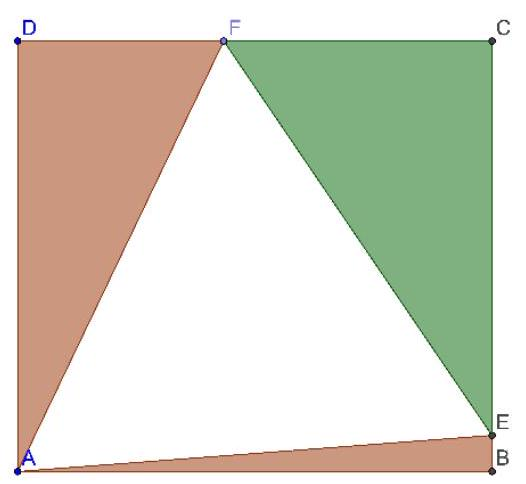
\includegraphics[max width=\textwidth, center]{2024_11_21_6cae607e190cc5a22142g-1}
  \item Punkt \(M\) jest środkiem przeciwprostokątnej \(A B\) trójkąta prostokątnego \(A B C\). Symetralna odcinka \(C M\) przecina proste \(A C\) i \(B C\) odpowiednio w punktach \(K\) i \(L\). Wykaż, że \(A K^{2}+B L^{2}=K L^{2}\)\\
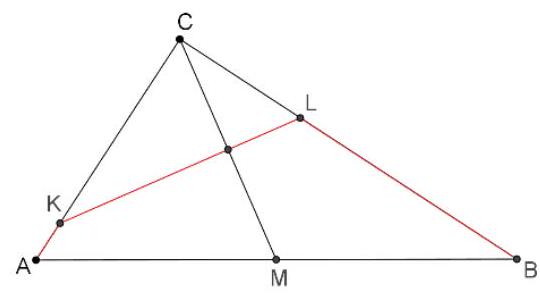
\includegraphics[max width=\textwidth, center]{2024_11_21_6cae607e190cc5a22142g-1(1)}
\end{enumerate}

\end{document}